\documentclass[table,xcolor=pdftex,dvipsnames]{beamer}\usepackage[]{graphicx}\usepackage[]{color}
%% maxwidth is the original width if it is less than linewidth
%% otherwise use linewidth (to make sure the graphics do not exceed the margin)
\makeatletter
\def\maxwidth{ %
  \ifdim\Gin@nat@width>\linewidth
    \linewidth
  \else
    \Gin@nat@width
  \fi
}
\makeatother

\definecolor{fgcolor}{rgb}{0.345, 0.345, 0.345}
\newcommand{\hlnum}[1]{\textcolor[rgb]{0.686,0.059,0.569}{#1}}%
\newcommand{\hlstr}[1]{\textcolor[rgb]{0.192,0.494,0.8}{#1}}%
\newcommand{\hlcom}[1]{\textcolor[rgb]{0.678,0.584,0.686}{\textit{#1}}}%
\newcommand{\hlopt}[1]{\textcolor[rgb]{0,0,0}{#1}}%
\newcommand{\hlstd}[1]{\textcolor[rgb]{0.345,0.345,0.345}{#1}}%
\newcommand{\hlkwa}[1]{\textcolor[rgb]{0.161,0.373,0.58}{\textbf{#1}}}%
\newcommand{\hlkwb}[1]{\textcolor[rgb]{0.69,0.353,0.396}{#1}}%
\newcommand{\hlkwc}[1]{\textcolor[rgb]{0.333,0.667,0.333}{#1}}%
\newcommand{\hlkwd}[1]{\textcolor[rgb]{0.737,0.353,0.396}{\textbf{#1}}}%
\let\hlipl\hlkwb

\usepackage{framed}
\makeatletter
\newenvironment{kframe}{%
 \def\at@end@of@kframe{}%
 \ifinner\ifhmode%
  \def\at@end@of@kframe{\end{minipage}}%
  \begin{minipage}{\columnwidth}%
 \fi\fi%
 \def\FrameCommand##1{\hskip\@totalleftmargin \hskip-\fboxsep
 \colorbox{shadecolor}{##1}\hskip-\fboxsep
     % There is no \\@totalrightmargin, so:
     \hskip-\linewidth \hskip-\@totalleftmargin \hskip\columnwidth}%
 \MakeFramed {\advance\hsize-\width
   \@totalleftmargin\z@ \linewidth\hsize
   \@setminipage}}%
 {\par\unskip\endMakeFramed%
 \at@end@of@kframe}
\makeatother

\definecolor{shadecolor}{rgb}{.97, .97, .97}
\definecolor{messagecolor}{rgb}{0, 0, 0}
\definecolor{warningcolor}{rgb}{1, 0, 1}
\definecolor{errorcolor}{rgb}{1, 0, 0}
\newenvironment{knitrout}{}{} % an empty environment to be redefined in TeX

\usepackage{alltt}

%\documentclass[table,xcolor=pdftex,dvipsnames, handout]{beamer}
%\usepackage{handoutWithNotes}
%\pgfpagesuselayout{4 on 1 with notes}[letterpaper,border shrink=5mm]

\usepackage{beamerthemesplit}
\usepackage[english]{babel}
\usepackage{amsmath}
\usepackage{amssymb}
\usepackage{amsthm}
\usepackage{verbatim}
\usepackage{graphpap}
\usepackage{epic}
\usepackage{pict2e} %To draw line with any slope
\usepackage{color}
\usepackage{natbib}
\usepackage{enumitem}
\usepackage{booktabs}
\usepackage{xcolor}
\usepackage{textcomp}
%\usepackage{movie15}

\bibliographystyle{ajae}

\newcommand{\p}{\partial}

\newcommand {\framedgraphic}[1] {
        \begin{center}
            \includegraphics[width=\textwidth,height=0.8\textheight,keepaspectratio]{#1}
        \end{center}
        \vspace{-1\baselineskip}
}

\usetheme{Boadilla}
\useoutertheme{shadow}
\usecolortheme{beaver}%seagull
\everymath{\color{blue}}
\everydisplay{\color{blue}}

\usefonttheme{professionalfonts}

\usepackage{hyperref}
\hypersetup{
   colorlinks = {true},
   urlcolor = {blue},
   linkcolor = {black},
   citecolor = {black},
   pdfborderstyle={/S/U/W 1},
   urlbordercolor = 0 0 1,
   citebordercolor = 1 1 1,
   filebordercolor = 1 1 1,
   linkbordercolor = 1 1 1,
   pdfauthor = {Sebastien Pouliot},
}

\widowpenalty=10000 % Avoid single line at the end of a page
\clubpenalty=10000  % Avoid single line at the bottom

\title[Futures]{Futures}
\author[Pouliot]{S\'{e}bastien Pouliot}
\institute{Iowa State University}
\date{Fall 2017}
\IfFileExists{upquote.sty}{\usepackage{upquote}}{}
\begin{document}

%%%%%%%%%%%%%%%%%%%%%%%%%%%%%%%%%%%%%%%%%%%%%%%%%%%%%%%%%%%%%%%%%%%%%%%%%%%%%%%%%%

\begin{frame}
\titlepage
\vspace{-0.4in}
\begin{center}
Lecture notes for Econ 235\\
\end{center}
\end{frame}

%%%%%%%%%%%%%%%%%%%%%%%%%%%%%%%%%%%%%%%%%%%%%%%%%%%%%%%%%%%%%%%%%%%%%%%%%%%%%%%%%%
\section{Introduction}

\begin{frame}{Definitions}
\begin{enumerate}[label=\textbullet]
  \item In the \emph{spot market} (cash market), buyers and sellers meet and transactions occur immediately (e.g. auction).
  \item A \emph{forward contract} specifies the price and time for the delivery of an item or a service.
\end{enumerate}
\end{frame}

%%%%%%%%%%%%%%%%%%%%%%%%%%%%%%%%%%%%%%%%%%%%%%%%%%%%%%%%%%%%%%%%%%%%%%%%%%%%%%%%%%

\begin{frame}{Definitions}
\begin{enumerate}[label=\textbullet]
  \item \emph{Futures} are similar to forward contracts as they both call for the delivery of an item or service at a specific time.
  \item However, the price of a futures contract is determined by the intersection of the demand and the supply for that contract and varies over time.
  \item Futures are traded in organized exchanges and are therefore standardized with respect to quantities, delivery location and time, product definition and quality.
  \item To read:
      \begin{enumerate}[label=\roman{*})]
          \item A Trader's Guide to Futures, available \href{http://www.cmegroup.com/education/a-traders-guide-to-futures.html}{online} and on Blackboard.
          \item Marketing Guide by Kevin Mcnew, old but still accurate, available on Blackboard.
      \end{enumerate}
\end{enumerate}
\end{frame}

%%%%%%%%%%%%%%%%%%%%%%%%%%%%%%%%%%%%%%%%%%%%%%%%%%%%%%%%%%%%%%%%%%%%%%%%%%%%%%%%%%



\begin{frame}{Price of December corn from 1990 to 2017}
\begin{knitrout}
\definecolor{shadecolor}{rgb}{0.969, 0.969, 0.969}\color{fgcolor}
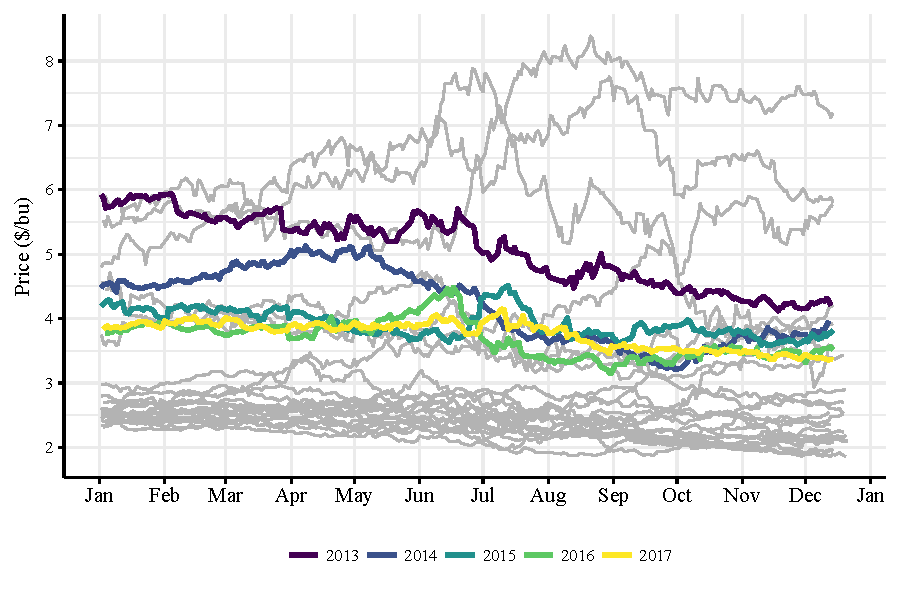
\includegraphics[width=\maxwidth]{figure/figure_corn_futures-1} 

\end{knitrout}
\end{frame}
%%%%%%%%%%%%%%%%%%%%%%%%%%%%%%%%%%%%%%%%%%%%%%%%%%%%%%%%%%%%%%%%%%%%%%%%%%%%%%%%%%
\begin{frame}{Price of November soybeans from 1990 to 2017}
\begin{knitrout}
\definecolor{shadecolor}{rgb}{0.969, 0.969, 0.969}\color{fgcolor}
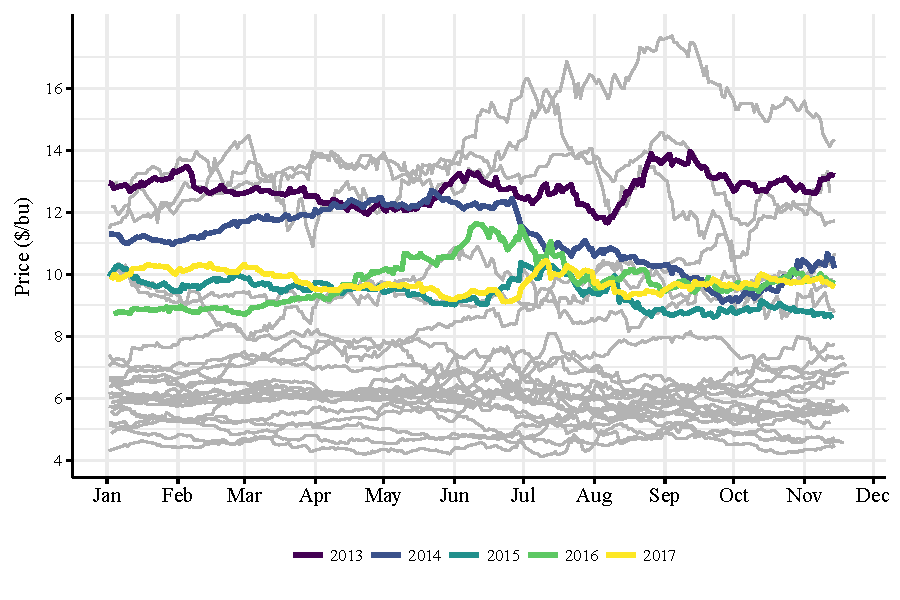
\includegraphics[width=\maxwidth]{figure/figure_soybeans_futures-1} 

\end{knitrout}
\end{frame}

%%%%%%%%%%%%%%%%%%%%%%%%%%%%%%%%%%%%%%%%%%%%%%%%%%%%%%%%%%%%%%%%%%%%%%%%%%%%%%%%%%

\begin{frame}{Origin of futures}
\begin{enumerate}[label=\textbullet]
  \item Futures, as we know them today, originated in the 19th century.
  \item In the United States, the Chicago Board of Trade was the first to organize futures trading.
  \item Chicago was the grain marketing center of the United States.
  \item Two factors motivated the development of futures contract:
     \begin{enumerate}[label=\roman{*})]
          \item Provide incentives to store grain;
          \item Correct large seasonal cash price changes.
      \end{enumerate}
\end{enumerate}
\end{frame}


%%%%%%%%%%%%%%%%%%%%%%%%%%%%%%%%%%%%%%%%%%%%%%%%%%%%%%%%%%%%%%%%%%%%%%%%%%%%%%%%%%

\begin{frame}{Futures exchanges}
\begin{enumerate}[label=\textbullet]
    \item Trade of futures contracts occurs in privately own exchanges.
    \item Most trades now occur through electronic trading.
    \item Federal (US Commodities Futures Trade Commission) and private regulations define the rules under which futures are traded.
    \item Historically, in the United States, futures have been traded at the \emph{Chicago Mercantile Exchange} (CME), the \emph{Chicago Board of Trade} (CBOT) and the New York Mercantile Exchange (NYME).
    \item In 2007, CME and CBOT merged to form CME Group Inc.
    \item CME Group Inc. bought NYME in 2008.
\end{enumerate}
\end{frame}

%%%%%%%%%%%%%%%%%%%%%%%%%%%%%%%%%%%%%%%%%%%%%%%%%%%%%%%%%%%%%%%%%%%%%%%%%%%%%%%%%%

\begin{frame}{What type of goods?}
\begin{enumerate}[label=\textbullet]
    \item Futures contract were first created for wheat and corn. Other storable agricultural commodities were later added.
    \item Futures for onions are illegal since the \emph{Onion Futures Act} of 1955 (price manipulation).
    \item Commodity exchanges added nonstorable agricultural commodities in the 1960s.
    \item Nonagricultural commodities (e.g. lumber and metals) were introduced in the 1970s.
    \item Financial futures (e.g. exchange rate, financial indices) were added in the 1980s.
\end{enumerate}
\end{frame}

%%%%%%%%%%%%%%%%%%%%%%%%%%%%%%%%%%%%%%%%%%%%%%%%%%%%%%%%%%%%%%%%%%%%%%%%%%%%%%%%%%

\begin{frame}{Price discovery}
\begin{enumerate}[label=\textbullet]
    \item One function of futures is to discover prices.
    \item The price of futures is determined by the intersection of demand and supply. It therefore summarizes all current market information and expectations.
    \item The cash price is linked to futures price through the basis. We will cover this in another section.
\end{enumerate}
\end{frame}


%%%%%%%%%%%%%%%%%%%%%%%%%%%%%%%%%%%%%%%%%%%%%%%%%%%%%%%%%%%%%%%%%%%%%%%%%%%%%%%%%%
\section{Specifications of futures contracts}

\begin{frame}{Specifications of futures contracts}
\begin{enumerate}[label=\textbullet]
    \item Exchanges define the parameters of futures contract.
\end{enumerate}
\vspace{-1.5\baselineskip}
\begin{table}
\caption{Some specifications of futures contracts for corn}
\scriptsize
\begin{tabular}{l l}
  \toprule
  Contract size & 5,000 bushels\\
  \addlinespace[0.075in]
  Deliverable grades & \parbox[t]{2.5in}{\#2 yellow at contract price, \#1 yellow at 1.5 cent/bushel premium, \#3 yellow at 1.5 cent/bushel discount}\\
  \addlinespace[0.075in]
  Price unit & Cents per bushel\\
  \addlinespace[0.075in]
  Tick size & 1/4 of one cent per bushel (\$12.50 per contract)\\
  \addlinespace[0.075in]
  Contract months/symbols & \parbox[t]{2.5in}{March (H), May (K), July(N), September (U) and December (Z)}\\
  \addlinespace[0.075in]
  Last trade date & \parbox[t]{2.5in}{The business day prior to the 15th calendar day of the contract month.}\\
  \addlinespace[0.075in]
  Last Delivery Date &  \parbox[t]{2.5in}{Second business day following the last trading day of the delivery month.}\\
  \bottomrule
\end{tabular}
\end{table}
\scriptsize
Source: \url{http://www.cmegroup.com/trading/agricultural/grain-and-oilseed/corn_contract_specifications.html}.
\end{frame}

%%%%%%%%%%%%%%%%%%%%%%%%%%%%%%%%%%%%%%%%%%%%%%%%%%%%%%%%%%%%%%%%%%%%%%%%%%%%%%%%%%
\begin{frame}{Specifications of futures contracts}
\begin{table}
\caption{Some specifications of futures contracts for soybeans}
\scriptsize
\begin{tabular}{l l}
  \toprule
  Contract size & 5,000 bushels\\
  \addlinespace[0.075in]
  Deliverable grades & \parbox[t]{2.5in}{\#2 Yellow at contract price, \#1 Yellow at a 6 cent/bushel premium, \#3 Yellow at a 6 cent/bushel discount}\\
  \addlinespace[0.075in]
  Price unit & Cents per bushel\\
  \addlinespace[0.075in]
  Tick size & 1/4 of one cent per bushel (\$12.50 per contract)\\
  \addlinespace[0.075in]
  Contract months/symbols & \parbox[t]{2.5in}{January (F), March (H), May (K), July (N), August (Q), September (U) and November (X)}\\
  \addlinespace[0.075in]
  Last trade date & \parbox[t]{2.5in}{The business day prior to the 15th calendar day of the contract month.}\\
  \addlinespace[0.075in]
  Last Delivery Date &  \parbox[t]{2.5in}{Second business day following the last trading day of the delivery month.}\\
  \bottomrule
\end{tabular}
\end{table}
\scriptsize
Source: \url{http://www.cmegroup.com/trading/agricultural/grain-and-oilseed/soybean_contract_specifications.html}.
\end{frame}

%%%%%%%%%%%%%%%%%%%%%%%%%%%%%%%%%%%%%%%%%%%%%%%%%%%%%%%%%%%%%%%%%%%%%%%%%%%%%%%%%%
\begin{frame}{Specifications of futures contracts}
\begin{table}
\caption{Some specifications of futures contracts for live cattle}
\scriptsize
\begin{tabular}{l l}
  \toprule
  Contract size & 40,000 pounds\\
  \addlinespace[0.075in]
  Deliverable grades & \parbox[t]{2.5in}{55\% Choice, 45\% Select, Yield Grade 3 live steers}\\
  \addlinespace[0.075in]
  Price unit & Cents per pound\\
 \addlinespace[0.075in]
  Tick size & \$.00025 per pound (=\$10 per contract)\\
  \addlinespace[0.075in]
  Contract months & \parbox[t]{2.5in}{February (G), April (J), June (M), August (Q), October (V), December (Z)}\\
  \addlinespace[0.075in]
  Last trade date & \parbox[t]{2.5in}{Last business day of the contract month, 12:00 p.m.}\\
  \addlinespace[0.075in]
  Last Delivery Date &  \parbox[t]{2.5in}{}\\
  \bottomrule
\end{tabular}
\end{table}
\scriptsize
Source: \url{http://www.cmegroup.com/trading/agricultural/livestock/live-cattle_contract_specifications.html}.
\end{frame}

%%%%%%%%%%%%%%%%%%%%%%%%%%%%%%%%%%%%%%%%%%%%%%%%%%%%%%%%%%%%%%%%%%%%%%%%%%%%%%%%%%%%%
\section{Who trades futures?}

\begin{frame}{Who trades futures?}
\begin{enumerate}[label=\textbullet]
      \item Trading futures requires a \emph{broker}, who is a person or a firm that handles futures trades for a commission.
      \item \emph{Hedgers }are buyers or sellers of the commodity that use futures to protect against price risk. We will cover hedging with futures in another section.
      \item \emph{Speculators}:
       \begin{enumerate}[label=-]
          \item These market participants trade futures because they foresee profits.
          \item Assume price risk from hedgers.
          \item Did Hillary Clinton make one hundred thousand dollars from an initial \$1,000 investment by trading cattle futures in 1978-79?
       \end{enumerate}
\end{enumerate}
\end{frame}


%%%%%%%%%%%%%%%%%%%%%%%%%%%%%%%%%%%%%%%%%%%%%%%%%%%%%%%%%%%%%%%%%%%%%%%%%%%%%%%%%%%%%

\begin{frame}{Who trades futures?}
\begin{enumerate}[label=\textbullet]
      \item \emph{Arbitrageurs}:
      \begin{enumerate}[label=-]
          \item Exploit short-term discrepancy in price relationship to gain profit.
       \end{enumerate}
      \item Speculators and arbitrageurs contribute to make markets efficient.
\end{enumerate}
\end{frame}

%%%%%%%%%%%%%%%%%%%%%%%%%%%%%%%%%%%%%%%%%%%%%%%%%%%%%%%%%%%%%%%%%%%%%%%%%%%%%%%%%%%%%

\begin{frame}{Position: definitions}
\begin{enumerate}[label=\textbullet]
      \item A trader is \emph{long in the cash market} if it has the capacity to deliver a commodity
       \begin{enumerate}[label=-]
           \item Gain if the price of the commodity \emph{increases}.
           \item For example, a farmer that has already planted corn is long in the cash market for corn.
       \end{enumerate}
      \item A trader is \emph{short in the cash market} if it has needs for a commodity.
        \begin{enumerate}[label=-]
           \item Gain if the price of the commodity \emph{decreases}.
           \item For example, a cattle feedlot that needs corn as a feed.
       \end{enumerate}
\end{enumerate}
\end{frame}


%%%%%%%%%%%%%%%%%%%%%%%%%%%%%%%%%%%%%%%%%%%%%%%%%%%%%%%%%%%%%%%%%%%%%%%%%%%%%%%%%%%%%

\begin{frame}{Position: definitions}
\begin{enumerate}[label=\textbullet]
       \item A \textbf{long} position in the futures market means that a trader has bought futures contracts:
       \begin{enumerate}[label=-]
          \item A buyer of a futures contract agrees to accept delivery of the asset in the future.
          \item Gain if the futures price \emph{increases}.
          \item Grain elevators or food producers may want to take a long position in the futures market to protect their costs of procurement against increase in the price of commodities.
       \end{enumerate}
      \item A \textbf{short} position in the futures means that a trader has sold futures contracts:
      \begin{enumerate}[label=-]
          \item A seller of a futures contract agrees to deliver the asset in the future.
          \item Gain if the futures price \emph{decreases}.
          \item Farmers may take a short position in the futures market to protect against decline in the price.
       \end{enumerate}
\end{enumerate}
\end{frame}

%%%%%%%%%%%%%%%%%%%%%%%%%%%%%%%%%%%%%%%%%%%%%%%%%%%%%%%%%%%%%%%%%%%%%%%%%%%%%%%%%%%%%

\begin{frame}{Definitions}
\begin{enumerate}[label=\textbullet]
      \item For most futures contracts, the product is never delivered as participants buy or sell offsetting positions.
      \item \emph{Open interest} is the number of open futures contract for which a trader remains obligated.
      \item Typically, traders offset their position before expiration.
        \begin{enumerate}[label=-]
          \item A trader that has a long position sells futures contract to offset his position.
          \item A trader that has a short position buys futures contract to offset his position.
        \end{enumerate}
\end{enumerate}
\end{frame}


%%%%%%%%%%%%%%%%%%%%%%%%%%%%%%%%%%%%%%%%%%%%%%%%%%%%%%%%%%%%%%%%%%%%%%%%%%%%%%%%%%%%%

\begin{frame}{Definitions}
\begin{enumerate}[label=\textbullet]
      \item \emph{Maturity} is the expiration date of a contract.
      \item \emph{Nearby} is the nearest active trading month of a futures.
\end{enumerate}
\end{frame}

%%%%%%%%%%%%%%%%%%%%%%%%%%%%%%%%%%%%%%%%%%%%%%%%%%%%%%%%%%%%%%%%%%%%%%%%%%%%%%%%%%
\section{Futures account}

\begin{frame}{Clearinghouse}
\begin{enumerate}[label=\textbullet]
    \item The clearinghouse is a corporation separated but associated with the exchange.
    \item The clearinghouse is responsible for recording each transaction, reconciling all trades and ensuring the integrity of each transaction.
    \item All trades must be cleared by the clearinghouse at the end of each day.
    \item The clearinghouse balances the books and manages the margin.
\end{enumerate}
\end{frame}

%%%%%%%%%%%%%%%%%%%%%%%%%%%%%%%%%%%%%%%%%%%%%%%%%%%%%%%%%%%%%%%%%%%%%%%%%%%%%%%%%%%%%


\begin{frame}{Purchasing and selling futures}
\begin{enumerate}[label=\textbullet]
      \item Trading futures requires having an account with a broker.
      \item Must first pass screening.
      \item A transaction on the futures market does not involve a direct exchange of money:
        \begin{enumerate}[label=-]
          \item The buyer of a contract does not pay any money to the seller;
          \item The seller of a contract does not receive any money from the buyer.
        \end{enumerate}
      \item The assumption is that buyers and sellers can offset their position by selling or buying futures contract. Thus, all that matters is that buyers and sellers have the money to cover losses in the event of unfavorable price changes.
      \item Provides leverage!
\end{enumerate}
\end{frame}


%%%%%%%%%%%%%%%%%%%%%%%%%%%%%%%%%%%%%%%%%%%%%%%%%%%%%%%%%%%%%%%%%%%%%%%%%%%%%%%%%%%%%


\begin{frame}{Initial margin}
\begin{enumerate}[label=\textbullet]
      \item For futures, gains and losses are realized every day.
      \item The only transfer of money that occurs is for daily gains or losses.
      \item Thus, it requires a margin where money can be removed or deposited to cover losses and realize gains.
      \item The value of the margins are set by the exchange and is determined in function of the futures prices and their variability.
      \item The \emph{initial margin} is the amount that must be deposited at the purchase or the sale of futures contracts.
      \item The initial margin equals 110\% of the value of the maintenance margin (\url{http://www.cmegroup.com/clearing/margins/}).
\end{enumerate}
\end{frame}

%%%%%%%%%%%%%%%%%%%%%%%%%%%%%%%%%%%%%%%%%%%%%%%%%%%%%%%%%%%%%%%%%%%%%%%%%%%%%%%%%%%%%

\begin{frame}{Maintenance margin and margin call}
\begin{enumerate}[label=\textbullet]
      \item The \emph{maintenance margin} is the minimum value that the margin account can take before money must be added to the margin account.
      \item If the amount of money in the account falls below the maintenance margin, then a \emph{margin call} is required to replenish the margin.
      \item In practice, it might not be easy to replenish your account margin. Do you have enough cash available? Is the bank willing to lend you money?
\end{enumerate}
\end{frame}

%%%%%%%%%%%%%%%%%%%%%%%%%%%%%%%%%%%%%%%%%%%%%%%%%%%%%%%%%%%%%%%%%%%%%%%%%%%%%%%%%%%%%

\begin{frame}{Initial margin and maintenance margin}
\begin{table}
\caption{Maintenance margins for selected agricultural commodities}
\scriptsize
\begin{tabular}{l c c}
  \toprule
  Product & Contract size& Maintenance margin  \\
  \addlinespace[0.075in]
  Corn & 5,000 bushels  & \$850 \\
  \addlinespace[0.075in]
  Soybean & 5,000 bushels & \$1,900 \\
  \addlinespace[0.075in]
  Wheat & 5,000 bushels  & \$1,200  \\
  \addlinespace[0.075in]
  Live cattle & 40,000 pounds & \$1,750  \\
  \addlinespace[0.075in]
  Lean hogs & 40,000 pounds & \$1,200  \\
  \bottomrule
\end{tabular}
\end{table}
\scriptsize
The margins change over time. These were the margins at the end of August 2017 and may have changed since. Source: \url{http://www.cmegroup.com/clearing/margins}.
\end{frame}


%%%%%%%%%%%%%%%%%%%%%%%%%%%%%%%%%%%%%%%%%%%%%%%%%%%%%%%%%%%%%%%%%%%%%%%%%%%%%%%%%%%%%

\begin{frame}{Example: long position}
\begin{enumerate}[label=\textbullet]
      \item Suppose that you go long on \textcolor[rgb]{1.00,0.00,0.00}{two} corn futures contracts for which the price is \textcent 400 per bushel on October 9.
      \item A futures contract is 5,000 bushels, with a current value of \$40,000 for two contracts.
      \item \emph{You do not pay \$40,000 unless you accept delivery of corn under your futures contract.}
      \item Suppose that the maintenance margin is \$1,400.
      \item The initial margin is \$1,540 (\$1,400$\times$110\%) for one futures contract of corn.
      \item The total amount of money required to buy two futures contract is therefore \$3,080 (2$\times$\$1,540).
      \item For the two corn futures contracts, the maintenance margin is \$2,800 (2$\times$\$1,400).
\end{enumerate}
\end{frame}

%%%%%%%%%%%%%%%%%%%%%%%%%%%%%%%%%%%%%%%%%%%%%%%%%%%%%%%%%%%%%%%%%%%%%%%%%%%%%%%%%%%%%

\begin{frame}{Example: long position}
\begin{enumerate}[label=\textbullet]
      \item Changes in the margin covers changes in the value of the futures contracts.
      \item Suppose that on October 10 that the price of the futures contract is \textcent 398 per bushel.
      \item This means that the total value of the contracts declines to \$39,800.
      \item The clearinghouse will remove \$200 to cover your loss and pay that amount to the owner of the short position on the contract.
      \item There is no margin call as the margin remains above \$2,800.
\end{enumerate}
\end{frame}

%%%%%%%%%%%%%%%%%%%%%%%%%%%%%%%%%%%%%%%%%%%%%%%%%%%%%%%%%%%%%%%%%%%%%%%%%%%%%%%%%%%%%

\begin{frame}{Example: long position}
\begin{table}
\caption{Account for \textcolor[rgb]{1.00,0.00,0.00}{two} units of corn futures - \textcolor[rgb]{1.00,0.00,0.00}{long position}}
\scriptsize
\begin{tabular}{l c c c c c c c}
  \toprule
  Date & \parbox[c]{0.5in}{\centering Price (\textcent/bushel)} & \parbox[c]{0.4in}{\centering Value (\$)} & \parbox[c]{0.40in}{\centering Margin (\$)}& \parbox[c]{0.55in}{\centering Daily gain or loss (\$)} & \parbox[c]{0.45in}{\centering Cumulative gain (\$)} & \parbox[c]{0.4in}{\centering Margin call (\$)}\\
  \midrule
  October 9 & 400 & 40,000 & 3,080 & 0 & 0 & 0\\
  October 10 & 398 & 39,800 & 2,880 & -200 & -200 & 0\\
  October 11 &  &  &   &  &  &  \\
  October 12 &  &  &   &  &  &  \\
  October 13 &  &  &   &  &  &  \\
  \bottomrule
\end{tabular}
\end{table}
\end{frame}


%%%%%%%%%%%%%%%%%%%%%%%%%%%%%%%%%%%%%%%%%%%%%%%%%%%%%%%%%%%%%%%%%%%%%%%%%%%%%%%%%%%%%

\begin{frame}{Example: long position}
\begin{enumerate}[label=\textbullet]
      \item Suppose that on October 11 that the price of the futures contract increase to \textcent402 per bushel.
      \item The margin increases by \$400 to \$3,280.
\end{enumerate}
\end{frame}

%%%%%%%%%%%%%%%%%%%%%%%%%%%%%%%%%%%%%%%%%%%%%%%%%%%%%%%%%%%%%%%%%%%%%%%%%%%%%%%%%%%%%

\begin{frame}{Example: long position}
\begin{enumerate}[label=\textbullet]
      \item On October 12, the price of the futures contract declines to \textcent395 per bushel.
      \item At that price, the margin falls below \$2,800 at \$2,580.
      \item Thus, it requires a margin call of \$500 to restore the margin at \$3,080.
\end{enumerate}
\end{frame}


%%%%%%%%%%%%%%%%%%%%%%%%%%%%%%%%%%%%%%%%%%%%%%%%%%%%%%%%%%%%%%%%%%%%%%%%%%%%%%%%%%%%%

\begin{frame}{Example: long position}
\begin{table}
\caption{Account for \textcolor[rgb]{1.00,0.00,0.00}{two} units of corn futures - \textcolor[rgb]{1.00,0.00,0.00}{long position}}
\scriptsize
\begin{tabular}{l c c c c c c}
  \toprule
  Date & \parbox[c]{0.5in}{\centering Price (\textcent/bushel)} & \parbox[c]{0.4in}{\centering Value (\$)} & \parbox[c]{0.40in}{\centering Margin (\$)}& \parbox[c]{0.55in}{\centering Daily gain or loss (\$)} & \parbox[c]{0.45in}{\centering Cumulative gain (\$)} & \parbox[c]{0.4in}{\centering Margin call (\$)}\\
  \midrule
  October 9 & 400 & 40,000 & 3,080 & 0 & 0 & 0\\
  October 10 & 398 & 39,800 & 2,880 & -200 & -200 & 0\\
  October 11 & 402  & 40,200  & 3,280 & 400 & 200 & 0\\
  October 12 & 395 & 39,500 & 3,080  & -700  & -500 & 500\\
  October 13 & 396 & 39,600 & 3,180 & 100 & -400 & 0 \\
  \bottomrule
\end{tabular}
\end{table}
\end{frame}


%%%%%%%%%%%%%%%%%%%%%%%%%%%%%%%%%%%%%%%%%%%%%%%%%%%%%%%%%%%%%%%%%%%%%%%%%%%%%%%%%%%%%

\begin{frame}{Example: short position}
\begin{enumerate}[label=\textbullet]
      \item Let's now assume instead that on October 9 you take a short position on \textcolor[rgb]{1.00,0.00,0.00}{three} corn futures contracts.
      \item The required initial margin for the three contracts is \$4,620 (3$\times$\$1,400$\times$110\%).
      \item The maintenance margin for the three contracts is \$4,200 (3$\times$\$1,400).
      \item With the short position, a margin call is not required because you gain from the decline in the price.
      \item Notice that the gains on the long position per unit of contract exactly equal the losses per contract on the short position.
\end{enumerate}
\end{frame}


%%%%%%%%%%%%%%%%%%%%%%%%%%%%%%%%%%%%%%%%%%%%%%%%%%%%%%%%%%%%%%%%%%%%%%%%%%%%%%%%%%%%%

\begin{frame}{Example: short position}
\begin{table}
\caption{Account for \textcolor[rgb]{1.00,0.00,0.00}{three} units of corn futures - \textcolor[rgb]{1.00,0.00,0.00}{short position}}
\scriptsize
\begin{tabular}{l c c c c c c}
  \toprule
  Date & \parbox[c]{0.5in}{\centering Price (\textcent/bushel)} & \parbox[c]{0.4in}{\centering Value (\$)} & \parbox[c]{0.40in}{\centering Margin (\$)}& \parbox[c]{0.55in}{\centering Daily gain or loss (\$)} & \parbox[c]{0.45in}{\centering Cumulative gain (\$)} & \parbox[c]{0.4in}{\centering Margin call (\$)}\\
  \midrule
  October 9 & 400 & 60,000 & 4,620 & 0 & 0 & 0\\
  October 10 & 398 & 59,700 & 4,920 & 300 & 300 & 0\\
  October 11 & 402 & 60,300  & 4,320 & -600 & -300 & 0\\
  October 12 & 395 & 59,250 & 5,370  & 1,050  & 750 & 0\\
  October 13 & 396 & 59,400 & 5,220 & -150 & 600 & 0 \\
  \bottomrule
\end{tabular}
\end{table}
\end{frame}

%%%%%%%%%%%%%%%%%%%%%%%%%%%%%%%%%%%%%%%%%%%%%%%%%%%%%%%%%%%%%%%%%%%%%%%%%%%%%%%%%%%%%
\section{Payoffs diagram}


\begin{frame}{Payoffs diagram}
\begin{enumerate}[label=\textbullet]
      \item A \emph{payoff diagram} shows gains and losses in function of futures price.
      \item The following payoff diagrams for one futures contract assumes that traders enter their position at \$4.00 per bushel.
\end{enumerate}
\end{frame}


%%%%%%%%%%%%%%%%%%%%%%%%%%%%%%%%%%%%%%%%%%%%%%%%%%%%%%%%%%%%%%%%%%%%%%%%%%%%%%%%%%%%



\begin{frame}{Payoffs diagram: long position}
\begin{knitrout}
\definecolor{shadecolor}{rgb}{0.969, 0.969, 0.969}\color{fgcolor}
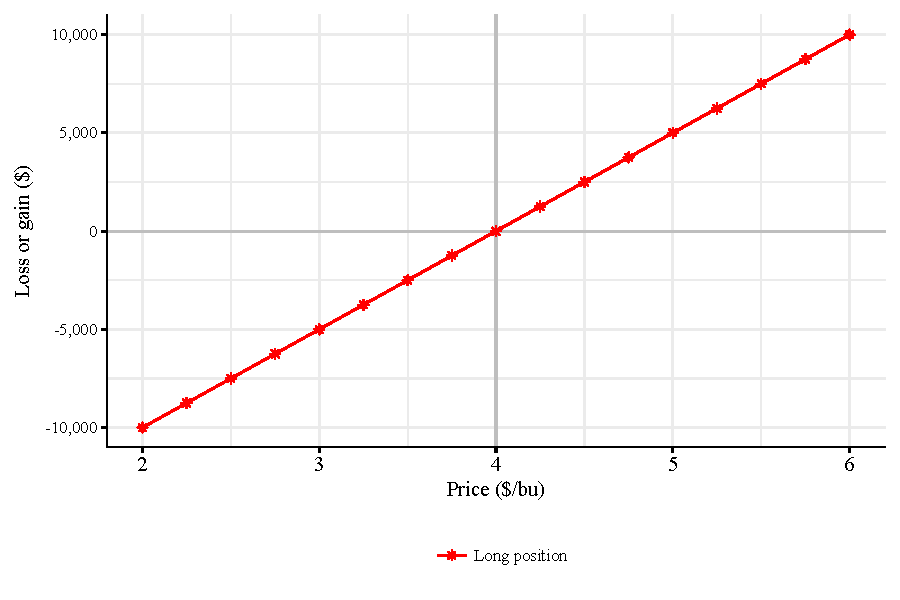
\includegraphics[width=\maxwidth]{figure/figure_long-1} 

\end{knitrout}
\end{frame}

%%%%%%%%%%%%%%%%%%%%%%%%%%%%%%%%%%%%%%%%%%%%%%%%%%%%%%%%%%%%%%%%%%%%%%%%%%%%%%%%%%%%%

\begin{frame}{Payoffs diagram: short position}
\begin{knitrout}
\definecolor{shadecolor}{rgb}{0.969, 0.969, 0.969}\color{fgcolor}
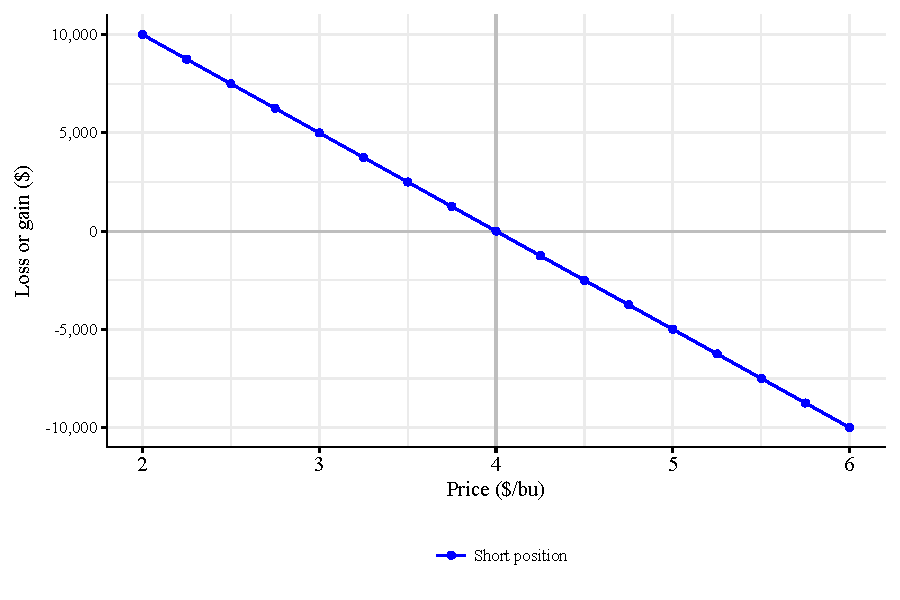
\includegraphics[width=\maxwidth]{figure/figure_short-1} 

\end{knitrout}
\end{frame}

%%%%%%%%%%%%%%%%%%%%%%%%%%%%%%%%%%%%%%%%%%%%%%%%%%%%%%%%%%%%%%%%%%%%%%%%%%%%%%%%%%%%%

\begin{frame}{Payoffs diagram}
\begin{knitrout}
\definecolor{shadecolor}{rgb}{0.969, 0.969, 0.969}\color{fgcolor}
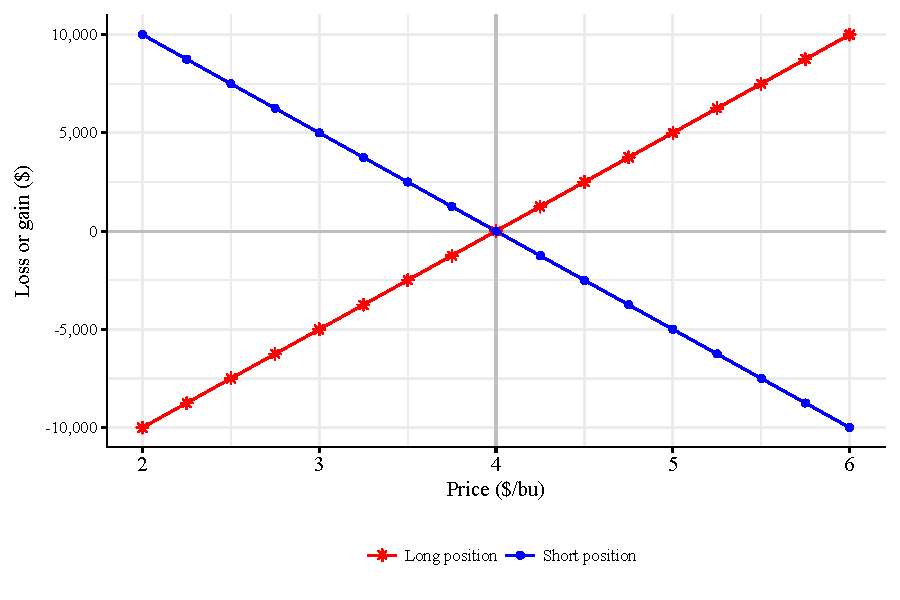
\includegraphics[width=\maxwidth]{figure/figure_position-1} 

\end{knitrout}
\end{frame}

%%%%%%%%%%%%%%%%%%%%%%%%%%%%%%%%%%%%%%%%%%%%%%%%%%%%%%%%%%%%%%%%%%%%%%%%%%%%%%%%%%%%%

\begin{frame}{Gains and losses}
\begin{enumerate}[label=\textbullet]
      \item On a per contract basis, gains on one position are losses on the opposite position.
      \item It is a zero sum game!
      \item For example, consider that the price of the futures contract equals 5.
\end{enumerate}
\end{frame}

%%%%%%%%%%%%%%%%%%%%%%%%%%%%%%%%%%%%%%%%%%%%%%%%%%%%%%%%%%%%%%%%%%%%%%%%%%%%%%%%%%%%%

\begin{frame}{Payoffs diagram for one unit of a futures contract}
\begin{knitrout}
\definecolor{shadecolor}{rgb}{0.969, 0.969, 0.969}\color{fgcolor}
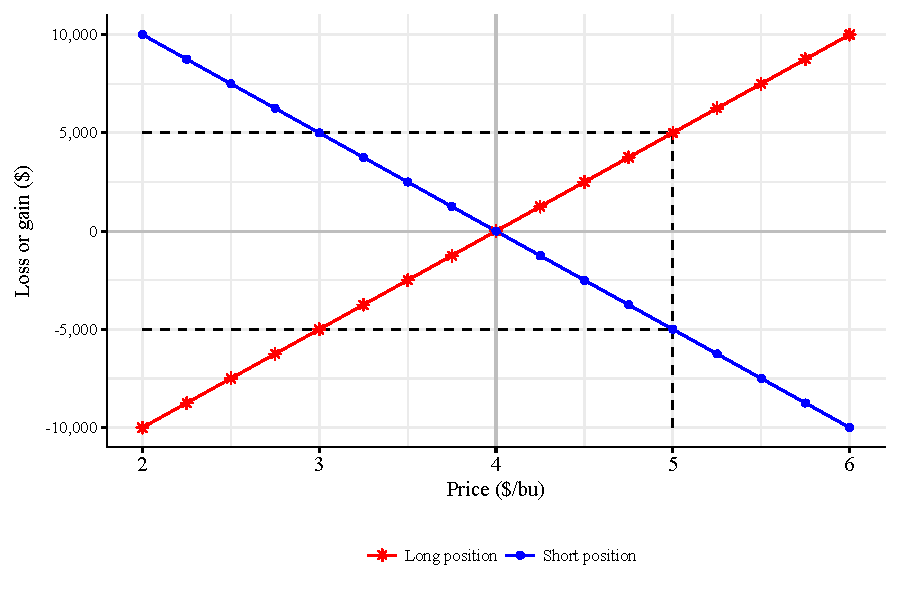
\includegraphics[width=\maxwidth]{figure/figure_position2-1} 

\end{knitrout}
\end{frame}

%%%%%%%%%%%%%%%%%%%%%%%%%%%%%%%%%%%%%%%%%%%%%%%%%%%%%%%%%%%%%%%%%%%%%%%%%%%%%%%%%%%%%
\section{Trading hours}


\begin{frame}{CME trading hours (CBOT)}
\begin{enumerate}[label=\textbullet]
      \item On weekdays, for corn, soybeans and other agricultural commodities, electronic trading occurs between between 19:00 and 7:45 and between 8:30 and 13:20, central time.
      \item Info on trading hours available at \url{http://www.cmegroup.com/trading_hours/commodities-hours.html}.
\end{enumerate}
\end{frame}

%%%%%%%%%%%%%%%%%%%%%%%%%%%%%%%%%%%%%%%%%%%%%%%%%%%%%%%%%%%%%%%%%%%%%%%%%%%%%%%%%%%%%
\section{Broker fees}

\begin{frame}{Broker fees (commission)}
\begin{enumerate}[label=\textbullet]
      \item Trading futures is not free.
      \item A broker generally asks for a small fee per transaction.
      \item The size of the fee varies depending on whether the broker offers some form of assistance such as market analysis.
      \item Your local grain elevator/coop may offer some brokerage services.
\end{enumerate}
\end{frame}

%%%%%%%%%%%%%%%%%%%%%%%%%%%%%%%%%%%%%%%%%%%%%%%%%%%%%%%%%%%%%%%%%%%%%%%%%%%%%%%%%%%%%

\begin{frame}{Example of broker fees}
    \framedgraphic{broker_fees.png}
Source was \url{http://www.tradestation.com/pricing/futures-pricing/futures-broker-comparison} but is no longer available.
\end{frame}

%%%%%%%%%%%%%%%%%%%%%%%%%%%%%%%%%%%%%%%%%%%%%%%%%%%%%%%%%%%%%%%%%%%%%%%%%%%%%%%%%%%%%
\section{Price limits}


\begin{frame}{Price limits}
\begin{enumerate}[label=\textbullet]
      \item To limit price volatility, exchanges set each day limits between which price for futures contract may vary.
      \item The parameters to set the limits are re-assessed quarterly.
      \item You can find details about trading limits here: \url{http://www.cmegroup.com/trading/equity-index/price-limit-guide.html}
\end{enumerate}
\end{frame}

%%%%%%%%%%%%%%%%%%%%%%%%%%%%%%%%%%%%%%%%%%%%%%%%%%%%%%%%%%%%%%%%%%%%%%%%%%%%%%%%%%%%%
\begin{frame}{Price limits: examples}
\begin{enumerate}[label=\textbullet]
      \item Corn:\$0.25 per bushel expandable to \$0.50 when the market closes at limit bid or limit offer. Source: \url{http://www.cmegroup.com/trading/agricultural/grain-and-oilseed/corn_contract_specifications.html}.
      \item Soybean: \$0.70 per bushel expandable to \$1.40 when the market closes at limit bid or limit offer. Source: \url{http://www.cmegroup.com/trading/agricultural/grain-and-oilseed/soybean_contract_specifications.html}.
\end{enumerate}
\end{frame}


%%%%%%%%%%%%%%%%%%%%%%%%%%%%%%%%%%%%%%%%%%%%%%%%%%%%%%%%%%%%%%%%%%%%%%%%%%%%%%%%%%%%%
\section{Terminology: Normal and inverted markets}

\begin{frame}{Definition: normal market}
\begin{enumerate}[label=\textbullet]
      \item In a \emph{normal market}, prices of futures contracts increase with their maturities.
      \item This holds in particular within a crop season.
      \item The increase in the price of futures contracts reflects the cost of storage and other costs of holding the commodity.
\end{enumerate}
\end{frame}

%%%%%%%%%%%%%%%%%%%%%%%%%%%%%%%%%%%%%%%%%%%%%%%%%%%%%%%%%%%%%%%%%%%%%%%%%%%%%%%%%%%%%

\begin{frame}{Definition: inverted market}
\begin{enumerate}[label=\textbullet]
      \item In an \emph{inverted market}, the prices of futures contracts decline with their maturities.
      \item This type of price pattern reflects conditions of the demand and supply for the commodity.
\end{enumerate}
\end{frame}

%%%%%%%%%%%%%%%%%%%%%%%%%%%%%%%%%%%%%%%%%%%%%%%%%%%%%%%%%%%%%%%%%%%%%%%%%%%%%%%%%%%%%

\begin{frame}{How are current markets?}
\begin{enumerate}[label=\textbullet]
      \item Futures contract price patterns reflect market's perception of future demand and supply.
      \item For agricultural commodities with seasonal patterns, markets will tend to be normal and inverted at the same time depending on the crop year.
        \begin{enumerate}[label=-]
          \item \href{http://www.barchart.com/commodityfutures/Corn_Futures/ZC}{Corn (Barchart)};
          \item \href{http://www.barchart.com/commodityfutures/Soybeans_Futures/ZS?search=ZS*}{Soybeans (Barchart)};
          \item \href{http://www.barchart.com/commodityfutures/Wheat_Futures/ZW?search=ZW*}{Wheat (Barchart)}.
        \end{enumerate}
      \item For commodities with less of a seasonal pattern, then the relationship between a futures contract price and its maturity will tend to be smoother.
          \begin{enumerate}[label=-]
            \item \href{http://www.barchart.com/commodityfutures/Live_Cattle_Futures/LE?search=LE*}{Live cattle (Barchart)};
            \item \href{http://www.barchart.com/commodityfutures/Lean_Hogs_Futures/HE?search=HE*}{Lean hogs (Barchart)};
            \item \href{http://www.barchart.com/commodityfutures/Crude_Oil_Futures/CL?search=CL*}{Crude oil (Barchart)};
            \item \href{http://www.barchart.com/commodityfutures/US_Dollar_Index_Futures/DX?search=DX*}{US dollar (Barchart)}.
          \end{enumerate}
\end{enumerate}
\end{frame}



%%%%%%%%%%%%%%%%%%%%%%%%%%%%%%%%%%%%%%%%%%%%%%%%%%%%%%%%%%%%%%%%%%%%%%%%%%%%%%%%%%%%%
%\section[References]{References}
%\renewcommand\refname{References}
%\def\newblock{References}
%\begin{frame}[allowframebreaks]{References}
%\bibliography{R:/users/pouliot/Papers/References}
%\bibliography{C:/Users/pouliot/Documents/Papers/References}
%\end{frame}


%%%%%%%%%%%%%%%%%%%%%%%%%%%%%%%%%%%%%%%%%%%%%%%%%%%%%%%%%%%%%%%%%%%%%%%%%%%%%%%%%%%%%

\end{document}

